
\documentclass[10pt]{article}
\usepackage{color}
\usepackage{makeidx}
\usepackage{graphicx}
\usepackage{underscore}
\usepackage{enumitem}
\newlist{longenum}{enumerate}{5}
\setlist[longenum,1]{label=\roman*)}
\setlist[longenum,2]{label=\alph*)}
\setlist[longenum,3]{label=\arabic*)}
\setlist[longenum,4]{label=(\roman*)}
\setlist[longenum,5]{label=(\alph*)}
\usepackage[section]{placeins}
\makeindex
\begin{document}
\begin{titlepage}
\centering
\huge{CMPE 315: Principles of VLSI Design Project Cover Page}
\vfill
\flushleft
\large{
Project Part 1\\
}
\vfill
Name: Brian Weber\\
Section: CMPE640 01\\
\vfill
Date Submitted: 11/22/2017
\vfill
\Large{TA / Grader Use Only:}\\
Late Submission Deduction (20\% per day):\\
\vspace{1cm}
Other Deductions:\\
\vspace{3cm}
Final Lab Grade:\\
\vspace{1cm}
Comments to student:\\
\vspace{5cm}
\end{titlepage}
\tableofcontents
    \section{Current Status of Code (Read Me)}
        Before getting into the bulk of the report I would like to write a short
summary of the status of my code. In it's current state, it works completely and
matches both test benches posted on Dr. Patel's website, with one small
exception: in the beginning of test bench 2, reset has to be asserted for an
extra clock cycle in order to reset the valid cells correctly. In addition, I
did not have time to clean up my code very much, so it is currently pretty
messy. I expect there are many floating signals and unused inputs/outputs of
entities that were abandoned as I rushed to fix bugs. I also have not
optimized most of my logic for cmos at this point. My first goal was to get the
code working, then polish later, but as it turns out, I didn't have any time for
polishing. To test, I have been hard coding timings into test benches, and
looking at the wave outputs. I do not have time to write different test benches,
so I will not have sample input and output files. Instead, I will include the
test benches that I have, along with the figures of the correct timing outputs.
\section{Entity Hierarchy}
    All entities are paired with architecture "structural".
    \begin{longenum}
    \item chip
        \begin{longenum}
        \item Counter
            \begin{longenum}
            \item rd_wr_hit_miss_reg
                \begin{longenum}
                \item dff_reset
                \item{Dlatch_Reset}
                \end{longenum}
            \item SR18
                \begin{longenum}
                \item dff_reset_high
                \end{longenum}
            \item dff_reset_high
            \item dff_reset
            \item srff
            \end{longenum}
        \item Cache_Block
            \begin{longenum}
            \item Cache_Cell_Row
                \begin{longenum}
                \item Cache_Cell_Valid
                    \begin{longenum}
                    \item SRlatch
                    \item tx
                    \end{longenum}
                \item Cache_Cell_Tag
                    \begin{longenum}    
                    \item Cache_Cell
                    \end{longenum}
                \item Cache_Cell_Data_Block
                    \begin{longenum}
                    \item Cache_Cell
                    \end{longenum}
                \end{longenum}
            \end{longenum}
        \item Decoder
        \item Hit_Miss
            \begin{longenum}
            \item Compare
            \end{longenum}
        \item Output_Enable
            \begin{longenum}
            \item tx
            \end{longenum}
        \item register8
            \begin{longenum}
            \item dff_reset
            \end{longenum}
        \end{longenum}
    \end{longenum}
\section{Chip}
    For the most part, this design sticks to the overall design shown in the
prompt. However, this design only uses one decoder to select which cache cell
will be operated on, rather than both a decoder and a multiplexor. Figure
 shows the overall design of the chip.
\section{Counter (State Machine)}
        The state machine is an entity called Counter, which is centered around
a shift register that keeps track of the number of clocks that pass after the
busy signal goes high. Depending on hit/miss status of each operation, different
things are done depending on the clock count after busy is set high. Another key
part of the state machine is a group of registers for storing both the inputs
from the cpu, and whether or not there was a hit or a miss. There is an entity
called rd_wr_hit_miss_reg that stores the operation (rd or write), as well as
whether it was a hit or miss, and outputs 4 separate lines. Figures
\ref{crdmiss}, \ref{crdhit}, \ref{cwrmiss}, and \ref{cwrhit} show input and
output waveforms that were generated from the test bench Counter_Test. These
figures prove the correct operation of the state machine. The definitions of the
signals are as follows:
\begin{itemize}
    \item s_reset: (Input) The global reset signal.
    \item s_clk: (Input) The global clock signal.
    \item s_busy: (Output) The global busy signal.
    \item s_start: (Input) The start signal from the CPU.
    \item s_cpu_dout_en: (Output) The signal which enables the transmission gate
from cache output to the CPU.
    \item s_cache_write: (Output) The signal which triggers all writes to the
cache.
    \item s_hit_miss: (Input) The signal from the Hit_Miss indicating whether
there is a hit or a miss.
    \item s_mem_enable: (Output) The signal that enables external memory.
    \item s_rd_wr: (Input) The rd_wr signal given from the CPU.
    \item s_rd_wr_o: (Output) A rd_wr signal that is sent to other modules after
the original rd_wr is latched.
    \item s_rm_wr_en: (Output) A signal that allows writing to the cache during
a read miss.
    \item s_wr_hit: (Output) A signal that is sent to other modules so they know
there was a write hit.
    \item s_write_[0:3]: (Output) Signals that select which block to be written
to during read a read miss.
\end{itemize} 

\begin{figure}[b]
    \centering
    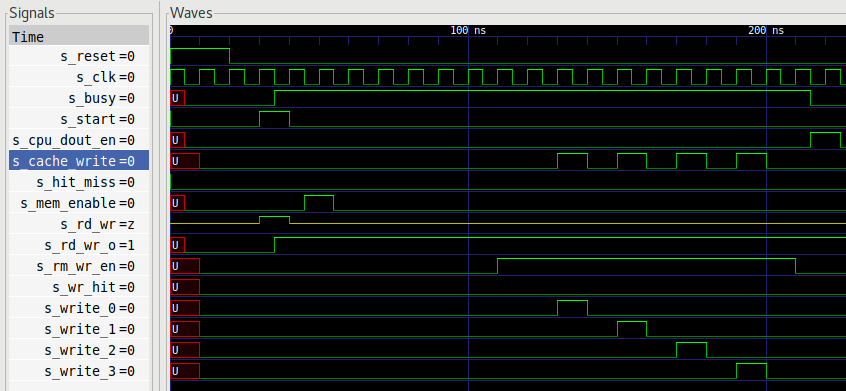
\includegraphics[width=\textwidth]{crm.png}
    \caption{Counter module timing during read miss.}
    \label{crdmiss}
\end{figure}

\begin{figure}
    \centering
    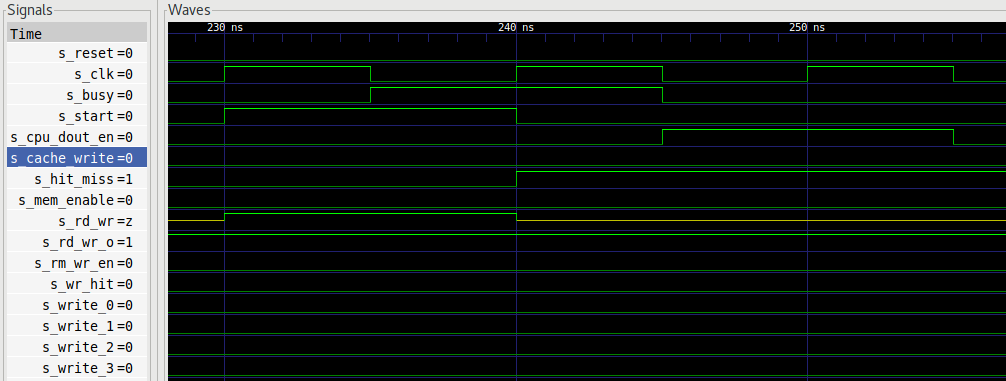
\includegraphics[width=\textwidth]{crh.png}
    \caption{Counter module timing during read hit.}
    \label{crdhit}
\end{figure}

\begin{figure}
    \centering
    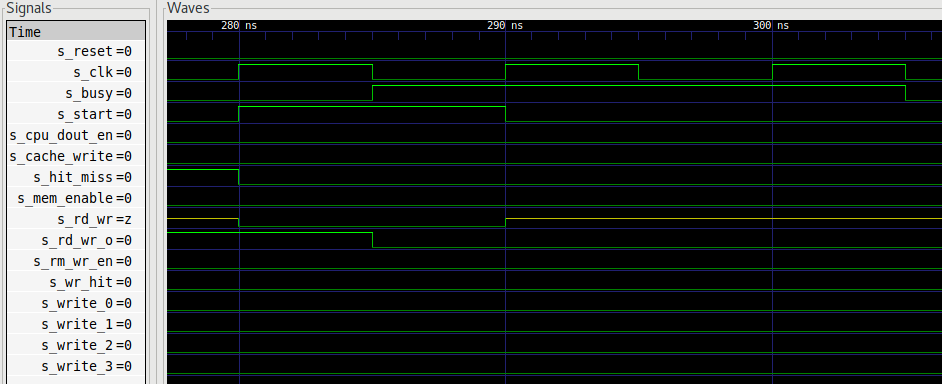
\includegraphics[width=\textwidth]{cwm.png}
    \caption{Counter module timing during write miss.}
    \label{cwrmiss}
\end{figure}

\begin{figure}
    \centering
    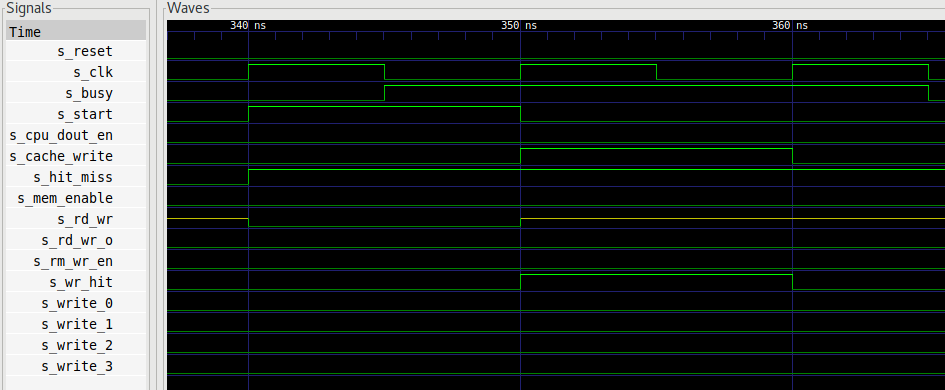
\includegraphics[width=\textwidth]{cwh.png}
    \caption{Counter module timing during write hit.}
    \label{cwrhit}
\end{figure}

\section{Cache_Block}
The cache block is a block of positive latch enabled Dlatches, indexed by the
cpu address. In front of each Dlatch is a transmission gate. The inputs and
outputs of each row all come from and lead to the same 8 bit bus, but only one row at a time can
be selected due to the Decoder module. This prevents conflicts on the outputs as
well as prevents more than one row from being written to at a time. The valid
cells are asynchronous sr latches, and are set while data is being written from
memory during a read miss. Tags are also set at this time. The valid and tag
bits are output as soon as a row is selected, however, for a byte to be
output, the internal rd_wr signal must be high, and a column must be selected.
Figure \ref{cb} shows a waveform diagram of the cache block. At 10 ns, the data
arrives at the input, the rd signal is turned on, and the row and column are
selected. At 15 ns, cache_write is turned on, writing the input data. Since rd
is on, the data shows on the output as well. At 15 ns, the tag and valid bits
are also set. Notice that after the rd signal turns off at 20 ns, the data
output becomes high impedence, however the tag and valid bits continue to
output. At 30 ns, different data is set at a different position. At 40 ns, the
old data is read, and at 45 seconds, the new data is read.

\begin{figure}
    \centering
    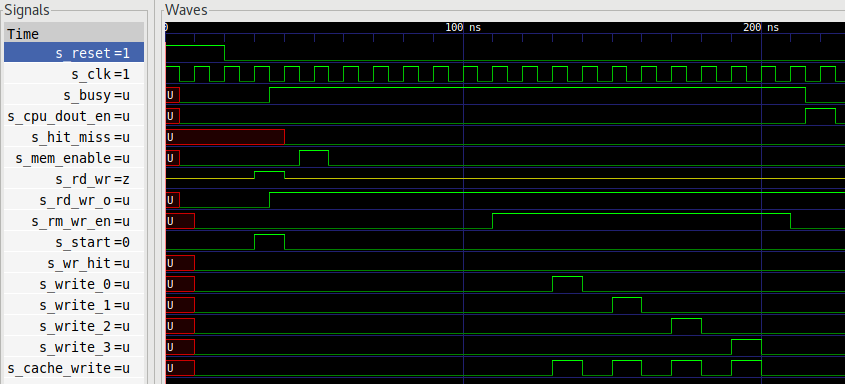
\includegraphics[width=\textwidth]{cb.png}
    \caption{Timing diagram showing the functionality of the cache_block.}
    \label{cb}
\end{figure}
\end{document}
